\coverchapter{Background}\label{ch:backgr}
\section{Combinatorics\label{sec:combinatorics}}
A \emph{bijection} from a set $A$ to a set $B$ is a function which relates each element of $A$ to a unique element of $B$ and vice versa. Suppose $A$ is the set of binary strings of length $n$ avoiding consecutive 1's and $B$ the set of subsets of $\{1,2,\ldots,n\}$ containing no consecutive numbers. By mapping each binary string $b_1b_2\dotsm b_n$ to the set containing $i$ if and only if $b_i=1$, we have a bijection. This bijection can be seen in \FigureRef{fig:bijection_example} for $n=3$.

\begin{figure}[ht!]
    \centering
    \begin{tikzpicture}[ele/.style={fill=black,circle,minimum width=.8pt,inner sep=1pt},every fit/.style={ellipse,draw,inner sep=35},scale=0.6, every node/.style={scale=0.6}]
    \draw[white] (0,0);
    \node[ele,label=left:$000$] (a1) at (0,4) {};    
    \node[ele,label=left:$100$] (a2) at (0,3) {};    
    \node[ele,label=left:$010$] (a3) at (0,2) {};
    \node[ele,label=left:$001$] (a4) at (0,1) {};
    \node[ele,label=left:$101$] (a5) at (0,0) {};
    
    \node[ele,label=right:$\emptyset$] (b1) at (6,4) {};
    \node[ele,label=right:$\set{1}$] (b2) at (6,3) {};
    \node[ele,label=right:$\set{2}$] (b3) at (6,2) {};
    \node[ele,label=right:$\set{3}$] (b4) at (6,1) {};
    \node[ele,label=right:$\set{1,3}$] (b5) at (6,0) {};
    
    \node[draw,fit= (a1) (a2) (a3) (a4) (a5),minimum width=4cm] {} ;
    \node[draw,fit= (b1) (b2) (b3) (b4) (b5),minimum width=4cm] {} ;  
    \draw[->,thick,shorten <=2pt,shorten >=2pt] (a1) -- (b1);
    \draw[->,thick,shorten <=2pt,shorten >=2] (a2) -- (b2);
    \draw[->,thick,shorten <=2pt,shorten >=2] (a3) -- (b3);
    \draw[->,thick,shorten <=2pt,shorten >=2] (a4) -- (b4);
    \draw[->,thick,shorten <=2pt,shorten >=2] (a5) -- (b5);
\end{tikzpicture}
    \caption{A bijection between binary strings of length 3 avoiding consecutive 1's and subsets of $\set{1,2,3}$ containing no consecutive numbers.}
    \label{fig:bijection_example}
\end{figure}

A \emph{combinatorial class} is a set $\mathcal{C}$ and a size function $\mathcal{C} \mapsto \N$ such that for all $n\in\N$, the set $\cset{c \in \mathcal{C}}{\text{size of $c$ is $n$}}$ is finite. We refer to an element of a combinatorial class, $c\in\mathcal{C}$, as a \emph{combinatorial object} and its size (or length) is denoted by $|c|$. We define $\mathcal{C}_n$ as the subset of $\mathcal{C}$ where size has been restricted to $n$ for some $n\in\N$. The set of words over a finite alphabet is an example of a combinatorial class where the length of a word serves as a size function. For a combinatorial class $\mathcal{C}$ we can write down an infinite sequence 
\[
    |\mathcal{C}_0|, |\mathcal{C}_1|, |\mathcal{C}_2|,\dotsc,|\mathcal{C}_n|,\dotsc
\]
where each term counts the number of elements of a fixed length. This sequence is the focal point of enumerative combinatorics. We might look for a formula for the terms, a recurrence relation or an asymptotic equivalence. If two combinatorial classes $\mathcal{C}$ and $\mathcal{D}$ share this sequence we say they are \emph{isomorphic}, denoted $\mathcal{C} \cong \mathcal{D}$. This is equivalent to the existence of a bijection between $\mathcal{C}$ and $\mathcal{D}$. Another way to present this sequence is with a power series $\sum_{i=0}^\infty |\mathcal{C}_i|z^i$ called a \emph{generating function} and famously described as a ``clothesline on which we hang up a sequence of numbers for display'' in Wilf \cite{wilf:gf}, referring to their refined closed form. For example the sequence of Fibonacci numbers $\left(f_i\right)_{i=0}^\infty$ has the generating function
\[
    \sum_{i=0}^\infty f_iz^i = 0 + z + z^2 + 2z^3 + 3z^4 + 5z^5 + 8z^6 + \dotsb = \frac{z}{1-z-z^2}.
\]
The \emph{symbolic method} in Flajolet and Sedgewick \cite{flajolet:ac} describes how combinatorial classes can be constructed. To that end, they define \emph{constructor}, \emph{combinatorial rule} and \emph{combinatorial specification}. We will demonstrate these concepts with an example. Consider a $2 \times n$ grid where each square can be raised or not as shown in \FigureRef{fig:raised_grid}. How many unique grids exist such that one can pass from left to right?

\begin{figure}[ht!]
    \centering
    {
\newcommand{\raised}[3]{\fill[white] #1;\fill[white] #2;\fill[white] #3;\draw #1;\draw #2;\draw #3;}

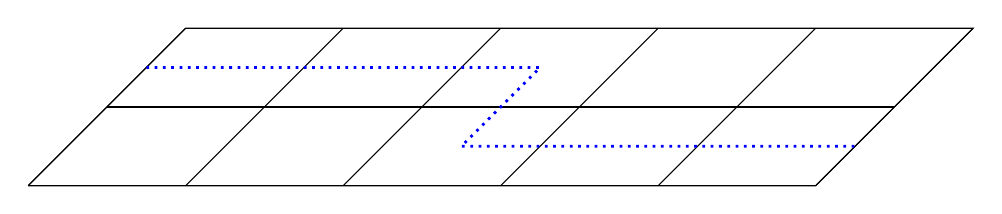
\begin{tikzpicture}[scale=2]
\def\rlvl{0.35}

% Grid
\draw (0,0) -- (1,1) -- (6,1) -- (5,0) -- (0,0);
\foreach \x in {0,1,...,5} {
    \draw (\x,0) -- (\x+1,1);
}
\draw (0.5,0.5) -- (5.5,0.5);

%Path
\draw[line width=0.35mm, blue, dotted] (0.75,0.75) -- (0.75+2.5,0.75) -- (0.75+2.5-0.5,0.75-0.5) -- (0.75+2.5-0.5+2.5,0.75-0.5);

% Raised squares
\raised{(1,0) rectangle (2,\rlvl)}{(2,0) -- (2.5,0.5) -- (2.5,0.5+\rlvl) -- (2,\rlvl)}{(2,\rlvl) -- (2.5,0.5+\rlvl) -- (1.5,0.5+\rlvl) -- (1,\rlvl)}
\raised{(1+2.5,0+0.5) rectangle (2+2.5,\rlvl+0.5)}{(2+2.5,0+0.5) -- (2.5+2.5,0.5+0.5) -- (2.5+2.5,0.5+\rlvl+0.5) -- (2+2.5,\rlvl+0.5)}{(2+2.5,\rlvl+0.5) -- (2.5+2.5,0.5+\rlvl+0.5) -- (1.5+2.5,0.5+\rlvl+0.5) -- (1+2.5,\rlvl+0.5)}
\raised{(1+2.5+1,0+0.5) rectangle (2+2.5+1,\rlvl+0.5)}{(2+2.5+1,0+0.5) -- (2.5+2.5+1,0.5+0.5) -- (2.5+2.5+1,0.5+\rlvl+0.5) -- (2+2.5+1,\rlvl+0.5)}{(2+2.5+1,\rlvl+0.5) -- (2.5+2.5+1,0.5+\rlvl+0.5) -- (1.5+2.5+1,0.5+\rlvl+0.5) -- (1+2.5+1,\rlvl+0.5)}
\end{tikzpicture}
}
    \caption{A grid of length $5$ with three raised squares and a path from left to right.}
    \label{fig:raised_grid}
\end{figure}

Let $G$ be the combinatorial class for passable grids. It is either the empty grid or contains at least one vertical slice. This is described by the admissible constructor disjoint union where a combinatorial class is split into nonintersecting parts. Now we have a combinatorial rule $G \cong \set{\varepsilon} \sqcup G_{\geq 1}$. In terms of generating functions this corresponds to addition, that is $G(x) = 1 + G_{\geq1}(x)$. Any valid grid consists of a combination of the vertical slices \gridN, \gridU\ and \gridD\ as one with both raised would block the path. We refer to a combinatorial object of length 1 as an \emph{atom}. The generating functions of the empty object and an atom are $1$ and $z$ respectively. Let $A$, $B$ and $C$ be the classes of passable grids starting with \gridN, \gridU\ and \gridD\ respectively and $D$ and $E$ the classes that can follow \gridU\ and \gridD\ respectively. Again we have a disjoint union $G_{\geq1} \cong A \sqcup B \sqcup C$. We define $\circ$ as the operator that prepends a vertical slice to all grids in a set. This is a Cartesian product, another admissible constructor denoted by $\times$ and in terms of generating functions corresponds to multiplication. Now we have $A \cong \gridN \circ G$, $B \cong \gridU \circ D$ and $C \cong \gridD \circ E$. Following \gridU\ can be anything that does not start by blocking the lower square, that is $D \cong \set{\varepsilon} \sqcup B \sqcup A$ and symmetrically we have $E \cong \set{\varepsilon} \sqcup C \sqcup A$. Now we have our specification, a system of rules with each nonfinite class on the left once, defining an unambiguous formal grammar as shown in \FigureRef{fig:gridtree}.

\begin{figure}[ht!]
    \centering
    {
\newcommand{\gridnodeempty}{%
\begin{tikzpicture}[scale=0.3, baseline=(current bounding box.center)]
\useasboundingbox (0,-3) rectangle (3,3);
			\draw[thick, rounded corners=3pt] (0,0) rectangle (3,3);
			\draw[pattern=north west lines, pattern color=lightgray]  (3,0) to[rounded corners=3pt] (0,0) to[rounded corners=3pt] (0,3) to[rounded corners=3pt] (3,3) to[rounded corners=3pt] cycle;
;
			    \end{tikzpicture}
}

\newcommand{\gridnodesingle}[1]{%
\begin{tikzpicture}[scale=0.3, baseline=(current bounding box.center)]
\useasboundingbox (0,-3) rectangle (3,3);
			\draw[thick, rounded corners=3pt] (0,0) rectangle (3,3);
			\node at (1.5, 1.5) {#1};
;
			    \end{tikzpicture}
}


\begin{tikzpicture}[scale=0.8, every node/.style={scale=0.8}]
    \node (root) at (0, 0) {\gridnodesingle{$G$}};
    \node (lvl_1_1) at (-1.5, -2.25) {\gridnodeempty};
    \node (lvl_1_2) at (1.5, -2.25) {\gridnodesingle{$G_{\geq1}$}};
    \node (lvl_2_1) at (-3, -4.5) {\gridnodesingle{$A$}};
    \node (lvl_2_2) at (1.5, -4.5) {\gridnodesingle{$B$}};
    \node (lvl_2_3) at (6, -4.5) {\gridnodesingle{$C$}};
    \node (lvl_3_1) at (-4,-6.75) {\gridnodesingle{\gridN}};
    \node (lvl_3_2) at (-2,-6.75) {\gridnodesingle{$G$}};
    \node (lvl_3_3) at (0.5,-6.75) {\gridnodesingle{$D$}};
    \node (lvl_3_4) at (2.5,-6.75) {\gridnodesingle{\gridU}};
    \node (lvl_3_5) at (5,-6.75) {\gridnodesingle{\gridD}};
    \node (lvl_3_6) at (7,-6.75) {\gridnodesingle{$E$}};
    \node (lvl_4_1) at (-1,-9) {\gridnodeempty};
    \node (lvl_4_2) at (0.5,-9) {\gridnodesingle{$B$}};
    \node (lvl_4_3) at (2,-9) {\gridnodesingle{$A$}};
    \node (lvl_4_4) at (5.5,-9) {\gridnodeempty};
    \node (lvl_4_5) at (7,-9) {\gridnodesingle{$C$}};
    \node (lvl_4_6) at (8.5,-9) {\gridnodesingle{$A$}};
    
    \ptedge{(root)}{(-0.5,1.2)}{(lvl_1_1)}{(-0.5,1.3)}
    \ptedge{(root)}{(-0.5,1.2)}{(lvl_1_2)}{(-0.5,1.3)}
    
    \ptedge{(lvl_1_2)}{(-0.5,1.2)}{(lvl_2_1)}{(-0.5,1.3)}
    \ptedge{(lvl_1_2)}{(-0.5,1.2)}{(lvl_2_2)}{(-0.5,1.3)}
    \ptedge{(lvl_1_2)}{(-0.5,1.2)}{(lvl_2_3)}{(-0.5,1.3)}
    
    \ptedge{(lvl_2_1)}{(-0.5,1.2)}{(lvl_3_1)}{(-0.5,1.3)}
    \ptedge{(lvl_2_1)}{(-0.5,1.2)}{(lvl_3_2)}{(-0.5,1.3)}
    \ptedge{(lvl_2_2)}{(-0.5,1.2)}{(lvl_3_3)}{(-0.5,1.3)}
    \ptedge{(lvl_2_2)}{(-0.5,1.2)}{(lvl_3_4)}{(-0.5,1.3)}
    \ptedge{(lvl_2_3)}{(-0.5,1.2)}{(lvl_3_5)}{(-0.5,1.3)}
    \ptedge{(lvl_2_3)}{(-0.5,1.2)}{(lvl_3_6)}{(-0.5,1.3)}
    
    \ptedge{(lvl_3_3)}{(-0.5,1.2)}{(lvl_4_1)}{(-0.5,1.3)}
    \ptedge{(lvl_3_3)}{(-0.5,1.2)}{(lvl_4_2)}{(-0.5,1.3)}
    \ptedge{(lvl_3_3)}{(-0.5,1.2)}{(lvl_4_3)}{(-0.5,1.3)}
    \ptedge{(lvl_3_6)}{(-0.5,1.2)}{(lvl_4_4)}{(-0.5,1.3)}
    \ptedge{(lvl_3_6)}{(-0.5,1.2)}{(lvl_4_5)}{(-0.5,1.3)}
    \ptedge{(lvl_3_6)}{(-0.5,1.2)}{(lvl_4_6)}{(-0.5,1.3)}
\end{tikzpicture}
}
    \caption{The grammar for passable $2\times n$ grids.}
    \label{fig:gridtree}
\end{figure}

This system of rules when interpreted with generating functions is a set of equations with functions as its unknowns. In our example we have
\[
    \systeme*{G(z) = 1 + G_{\geq1}(z), G_{\geq1}(z) = A(z) + B(z) + C(z),A(z) = zG(z), B(z) = zD(z), C(z) = zE(z), D(z) = 1+B(z)+A(z), E(z) = 1+C(z)+A(z)}
\]
and solving for $G(z)$ gives $G(z) = \frac{1+z}{1-2z-z^2}$. The Taylor series for this function, at $z=0$, is
\[
    \sum_{i=0}^\infty \frac{G^{(i)}(0)}{i!}z^i = 1+3z+7z^2+17z^3+ 41z^4 + 99z^5 + \dotsm
\]
which corresponds to the number of grids for each size e.g., there are 17 and 99 unique passable $2\times3$ and $2\times5$ grids respectively. We can even go further with some calculus and find the exact formula, $|G_n| = \frac{\left(1+\sqrt{2}\right)^{n+1} + \left(1-\sqrt{2}\right)^{n+1}}{2}$. This is not always the case and depends on the type of generating function we have.

In the context of this paper, we will usually refer to combinatorial classes as just classes and the same goes for combinatorial specifications and rules. We also assume all constructors to be admissible.

\section{Permutations\label{sec:permutations}}
A \emph{permutation} $\pi$ is a one-to-one correspondence between a set and itself. In our context, the set in question is $[n] = \{1,2,\dotsc,n\}$. We adopt a one line notation for permutations, $\pi = \pi_1 \pi_2 \dotsm \pi_n$ where $\pi_i = j$ if $i$ maps to $j$. The permutation $1423$ maps $\{1,2,3,4\}$ to itself. This correspondence can be seen in \FigureRef{fig:perm_example} as well as a geometric representation of the permutation which displays the points $\cset{(i,\pi(i))}{i \in [n]}$ in the Cartesian plane.

\begin{figure}[ht!]
    \centering
    \begin{tikzpicture}[ele/.style={fill=black,circle,minimum width=.8pt,inner sep=1pt},every fit/.style={ellipse,draw,inner sep=15},scale=0.6, every node/.style={scale=0.6}]
    \draw[white] (0,0);
    \node[ele,label=left:$1$] (a1) at (0,4) {};    
    \node[ele,label=left:$2$] (a2) at (0,3) {};    
    \node[ele,label=left:$3$] (a3) at (0,2) {};
    \node[ele,label=left:$4$] (a4) at (0,1) {};
    
    \node[ele,,label=right:$1$] (b1) at (4,4) {};
    \node[ele,,label=right:$2$] (b2) at (4,3) {};
    \node[ele,,label=right:$3$] (b3) at (4,2) {};
    \node[ele,,label=right:$4$] (b4) at (4,1) {};
    
    \node[draw,fit= (a1) (a2) (a3) (a4),minimum width=2cm] {} ;
    \node[draw,fit= (b1) (b2) (b3) (b4),minimum width=2cm] {} ;  
    \draw[->,thick,shorten <=2pt,shorten >=2pt] (a1) -- (b1);
    \draw[->,thick,shorten <=2pt,shorten >=2] (a2) -- (b4);
    \draw[->,thick,shorten <=2pt,shorten >=2] (a3) -- (b2);
    \draw[->,thick,shorten <=2pt,shorten >=2] (a4) -- (b3);
\end{tikzpicture}
\hspace{2cm}
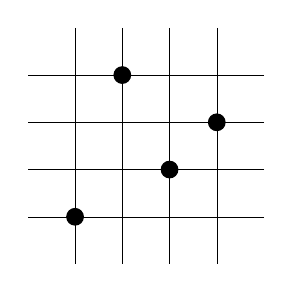
\begin{tikzpicture}[,scale=0.6, every node/.style={scale=0.6}]
        \foreach \x in {1,...,4} {
                \draw[ultra thin] (\x,5)--(\x,0);
                \draw[ultra thin] (5,\x)--(0,\x);
        }
        \draw[fill=black] (1,1) circle (5pt);
        \draw[fill=black] (2,4) circle (5pt);
        \draw[fill=black] (3,2) circle (5pt);
        \draw[fill=black] (4,3) circle (5pt);
\end{tikzpicture}
    \caption{The mapping and graphical representation of the permutation $1423$.}
    \label{fig:perm_example}
\end{figure}

A permutation on $[n]$ is said to be of length $n$ and $\mathcal{S}_n$ is the set of all permutations of length $n$. The set of permutations of length 3 is $\mathcal{S}_3 = \{123,132,213,231,312,321\}$. There is a permutation of length $0$, namely the empty permutation, denoted $\varepsilon$. This is the unique map from $\emptyset$ to $\emptyset$. The set of all permutations is denoted by $\mathcal{S}$. It is a combinatorial class since $\mathcal{S}_n$ is finite for all $n\in\N$, containing $n!$ elements.

The $S$-\emph{subsequence} of a permutation $\pi \in \mathcal{S}_n$ for $S\subseteq [n]$ is the sequence $\sseq{S}{\pi}=\pi_{i_1}\pi_{i_2}\dotsb \pi_{i_{|S|}}$ \todo{JSE: revisit this notation, $\Xi_S\pi$} where $\{i_1,i_2,\dotsc,i_{|S|}\} = S$ and $i_1 < i_2 < \dotsb < i_{|S|}$. Given an $S$-subsequence $\gamma$ of a permutation $\pi \in \mathcal{S}_n$, its \emph{standardization}, $\st{\gamma}$, is the sequence where the $i^\text{th}$ largest entry has been replaced by $i$. Let $\pi = 41253 \in \mathcal{S}_5$ and $S=\{1,3,4\}$, then $\st{\sseq{S}{\pi}} = \st{425} = 213$.

Given two permutations $\pi \in \mathcal{S}_n$ and $\sigma \in \mathcal{S}_k$ we say that $\pi$ \emph{contains} $\sigma$, denoted $\contains{\pi}{\sigma}$, if there exists a subset $S \subseteq [n]$ such that $\st{\sseq{S}{\pi}} = \sigma$. If $\pi$ does not contain $\sigma$, it \emph{avoids} it. In the context of containment, we usually refer to the contained permutation as a \emph{pattern} and that permutations contain or avoid a pattern. The permutation $356214$ contains the pattern $4213$ since $\st{\sseq{\{2, 4, 5, 6\}}{356214}} = \st{5214} = 4213$. It, however, avoids the pattern $1432$ since $1432 \notin \cset{\st{\sseq{S}{356214}}}{S \subseteq [6]}$. An occurrence of $4213$ in $356214$ can be seen in \FigureRef{fig:pattern_containment}.

\begin{figure}[ht!]
    \centering
    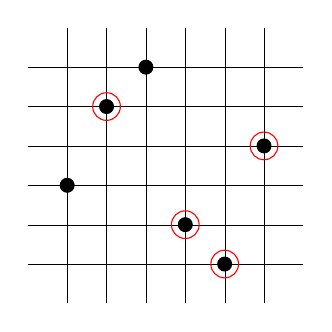
\begin{tikzpicture}[scale=.5,baseline=(current bounding box.center)]
    \foreach \x in {1,...,6} {
        \draw[ultra thin] (\x,0)--(\x,7); %vline
        \draw[ultra thin] (0,\x)--(7,\x); %hline
    }
    \draw[fill=black] (1,3) circle (5pt);
    \draw[fill=black] (2,5) circle (5pt);
    \draw[fill=black] (3,6) circle (5pt);
    \draw[fill=black] (4,2) circle (5pt);
    \draw[fill=black] (5,1) circle (5pt);
    \draw[fill=black] (6,4) circle (5pt);
    \draw[red] (2,5) circle (10pt);
    \draw[red] (4,2) circle (10pt);
    \draw[red] (5,1) circle (10pt);
    \draw[red] (6,4) circle (10pt);
\end{tikzpicture}
    \caption{The permutation $356214$ with an occurrence of $4213$ circled.}
    \label{fig:pattern_containment}
\end{figure}

A set of permutation $\Pi$ is \emph{closed downwards} with respect to containment if 
\[
    \bigcup_{\pi \in \Pi}\cset{\sigma \in \mathcal{S}}{\contains{\pi}{\sigma}} \subseteq \Pi.
\]
A set of permutations that is closed downwards is called a \emph{permutation class}. The set $\{\varepsilon, 1, 12, 123\}$ is closed downwards since all patterns contained in each of its elements belongs to the set. We can extend this set to include all increasing permutations, $\set{\varepsilon, 1, 12, 123, 1234, \dotsc}$ and it is still closed downwards. Both sets are therefore permutation classes.

A permutation $\pi$ \emph{avoids} a set of permutations $\Pi$ if it avoids every $\sigma \in \Pi$. It \emph{contains} $\Pi$ if it does not avoid it, that is, it contains any permutation of $\Pi$. Let $\Av{\Pi} = \cset{\pi \in \mathcal{S}}{\pi \text{ avoids } \Pi}$. We may abuse this notation by omitting the brackets, writing $\Av{\sigma_1,\sigma_2}$ instead of $\Av{\set{\sigma_1,\sigma_2}}$. Let $\textsf{Av}_n\left(\Pi\right) = \cset{\pi \in \Av{\Pi}}{|\pi| = n}$ for $n\in\N$.

A set of permutations $\mathcal{B}$ is called a \emph{basis} if for all $\pi\in\mathcal{B}$ there does not exist a $\sigma \in \mathcal{B} \setminus \set{\pi}$ such that $\contains{\pi}{\sigma}$. The set $\{12,21\}$ is a basis while $\{12,231\}$ is not since $\contains{231}{12}$. Any permutation class can be described in terms of a basis. For example $\{\varepsilon,1,12,123\} = \Av{21, 1234}$ and $\{\varepsilon, 1, 12, 123, 1234,\dotsc\} = \Av{21}$.


\section{Gridded permutations\label{sec:griddedpermutations}}
A \emph{cell} $(a,b) \in \N^2$ is the region within $[0,\infty)^2$ defined by $[a, a+1) \times [b, b+1).$ A pair $(\pi,P) = (\pi_1\pi_2\dotsb\pi_n, ((a_1,b_1),(a_2,b_2),\dotsc,(a_n,b_n)))$ where $P$ is a $n$-tuple of cells and $\pi$ is a permutation is called a \emph{gridded permutation} of length $n$ if for all $i,j \in [n]$, $i<j$ implies $a_i \leq a_j$ and $\pi_i < \pi_j$ implies $b_i \leq b_j$. A more detailed definition is given by Albert \cite{albert2012geometric}. We refer to $P$ as the \emph{positions} of the gridded permutation and $\pi$ as the \emph{underlying permutation}. We use a one line notation for gridded permutations $\pi = \pi_1^{(a_1,b_1)}\pi_1^{(a_2,b_2)}\dotsb\pi_n^{(a_n,b_n)}$ where we can exclude all but the last position of consecutive occurrences of the same position. The gridded permutation $87^{(0,2)}1^{(1,0)}6^{(1,2)}2^{(1,0)}4^{(3,1)}3^{(3,0)}5^{(4,2)}$ can be seen in \FigureRef{fig:gridded_perm}.

\begin{figure}[ht!]
    \centering
    \input{graphics/gridded_perm}
    \caption{The gridded permutation $87^{(0,2)}1^{(1,0)}6^{(1,2)}2^{(1,0)}4^{(3,1)}3^{(3,0)}5^{(4,2)}$.}
    \label{fig:gridded_perm}
\end{figure}

We extend the definition of $S$-subsequences to gridded permutations so the sequence produced, $\sseq{S}{\pi}$, contains elements of the underlying permutation and positions. Given this extension, we can also extend the standardization of an $S$-subsequence of a gridded permutation to be applied only to the underlying permutation. For example, given a gridded permutation $\pi = 1^{(0,0)}5^{(1,2)}2^{(2,0)}43^{(2,1)}$ and $S=\set{1,2,5}$ we have $\st{\sseq{S}{\pi}} = \st{1^{(0,0)}5^{(1,2)}3^{(2,1)}} = 1^{(0,0)}3^{(1,2)}2^{(2,1)}$. Using the extended definition of standardization we can also extend containment and avoidance to gridded permutations, for both a single and sets of gridded permutations. For example, the gridded permutation $1^{(0,0)}5^{(1,2)}2^{(2,0)}43^{(2,1)}$ contains $1^{(0,0)}2^{(2,0)}3^{(2,1)}$ but avoids $1^{(0,0)}23^{(2,1)}$.

Let $\mathcal{G}$ be the set of all gridded permutations and $\mathcal{G}_n$ its subset with only gridded permutations of length $n$. The set $\mathcal{G}$ is not a combinatorial class since $\mathcal{G}_n$ is infinite for all $n \in \Z^+$ having infinitely many cells to choose from. If we restrict the choice of cells to be finite, then so are the gridded permutations we can form. Let $\mathcal{G}^{(c,r)}$ be the set of gridded permutation with positions in $\{0,1,\dotsc,c-1\} \times \{0,1,\dotsc,r-1\}$ and $\mathcal{G}^{(c,r)}_n = \cset{\pi \in \mathcal{G}^{(c,r)}}{|\pi| = n}$. The set $\mathcal{G}^{(c,r)}$ is a combinatorial class and we extend the definitions of $\textsf{Av}^{(c,r)}\left(\Pi\right)$ and $\textsf{Av}_n^{(c,r)}\left(\Pi\right)$ to gridded permutations.

\section{Tilings\label{sec:tilings}}
A \emph{tiling} is a triple $\mathcal{T} = ((c,r), \mathcal{O}, \set{\mathcal{R}_1,\mathcal{R}_2,\dotsc,\mathcal{R}_k})$ where $(c,r) \in \Z^+ \times \Z^+$, $\mathcal{O} \subseteq \mathcal{G}^{(c,r)}$ and $\mathcal{R}=\set{\mathcal{R}_1,\mathcal{R}_2,\dotsc,\mathcal{R}_k} \subseteq \left(\mathcal{G}^{(c,r)}\right)^k$ are called \emph{dimension}, \emph{obstructions} and \emph{requirements} respectively. The gridded permutations in $\mathcal{G}^{(c,r)}$ that avoid $\mathcal{O}$ and contain $\mathcal{R}_1,\dotsc,\mathcal{R}_k$ make up the combinatorial class $\textsf{Grid}(\mathcal{T})$. A more detailed definition is given by Bean \cite{BeanPhd:phd}. An example of a tiling can be seen in \FigureRef{fig:tiling_example} where obstructions are red and requirements blue. Positions with $12$ and $21$ obstruction and a $1$ requirement are represented with a larger black point. \todo{JSE: black \& white - ify}

\begin{figure}[ht!]
    \centering
    {
% rect
%\newcommand{\reqpnt}[3]{\fill[blue] (#1-#3,#2-#3) rectangle (#1+#3,#2+#3);}
% donut
%\newcommand{\reqpnt}[3]{\fill[blue] (#1,#2) circle (#3); \fill[white] (#1,#2) circle (#3 * 0.5);}
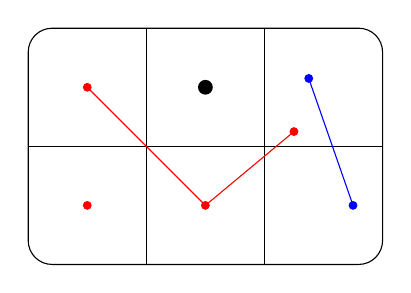
\begin{tikzpicture}[scale=0.75, every node/.style={scale=0.75}]
    \def\spnt{0.075} % Size of smaller points
    \def\lpnt{0.125} % Size of larger points
    \draw[rounded corners=2ex] (0,0) rectangle (6,4);
    \draw (2.0, 4) -- (2.0, 0);
    \draw (4.0, 4) -- (4.0, 0);
    \draw (0, 2) -- (6.0, 2);
    \fill[red] (1, 3) circle (\spnt);
    \fill[red] (1, 1) circle (\spnt);
    \fill[red] (3, 1) circle (\spnt);
    \fill[red] (4.5, 2.25) circle (\spnt);
    \draw[red] (1, 3) -- (3,1) -- (4.5,2.25);
    \fill (3,3) circle (\lpnt);
    \draw[blue] (4.75, 3.15) -- (5.5,1);
    \fill[blue] (4.75, 3.15) circle (\spnt);
    \fill[blue] (5.5, 1) circle (\spnt);
    %\reqpnt{4.75}{3.15}{\spnt*1.2}
    %\reqpnt{5.5}{1}{\spnt*1.2}
\end{tikzpicture}
}
    \caption{A $3 \times 2$ tiling with $\mathcal{R} = \set{\set{1^{(1,1)}}, \set{2^{(1,1)}1^{(2,0)}}}$ and $\mathcal{O}$ consisting of $1^{(0,0)}$, $12^{(1,1)}$, $21^{(1,1)}$ and $3^{(0,1)}1^{(1,0)}2^{(2,1)}$.}
    \label{fig:tiling_example}
\end{figure}

Typically when we want to enumerate $\Av{132}$ we start with a disjoint union constructor as its either empty or contains a largest point. If it contains a largest point, it must still avoid 132 on either side. Furthermore the elements to the left of the largest point must be greater than those to its right or you have an occurrence of $132$ with the largest point. This is important since it allows us to uniquely map the elements to the right of the largest point from the rule. Now we have a specification
\begin{align*}
\Av{132} &\cong \set{\varepsilon} \sqcup \textsf{Av}_{\geq1}(132)\\
\textsf{Av}_{\geq1}(132) &\cong \Av{132} \times \set{\point{0.1}} \times \Av{132}
\end{align*}
and a generating function $\frac{1-\sqrt{1-4z}}{2z}$. This was a simple example but given different classes and constructors, we can end up with classes that are hard to describe accurately. This is the purpose of tilings, a sort of language to describe classes with more complicated permutation constraints or limited parts of permutations. For example we can describe $\textsf{Av}_{\geq1}(132)$ with the tiling seen in \FigureRef{fig:tiling132}.

\begin{figure}[ht!]
    \centering
    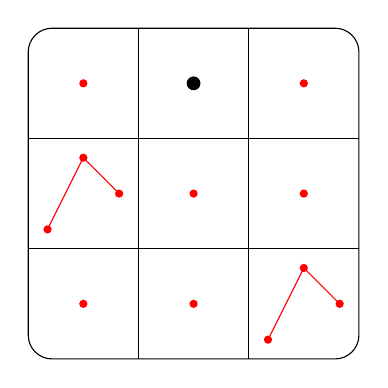
\begin{tikzpicture}[scale=0.7, every node/.style={scale=0.7}]
    \def\spnt{0.075} % Size of smaller points
    \def\lpnt{0.125} % Size of larger points
    \draw[rounded corners=2ex] (0,0) rectangle (6,6);
    \draw (2.0, 6) -- (2.0, 0);
    \draw (4.0, 6) -- (4.0, 0);
    \draw (0, 2) -- (6.0, 2);
    \draw (0, 4) -- (6.0, 4);
    \fill[red] (1, 5) circle (\spnt);
    \fill[red] (1, 1) circle (\spnt);
    \fill[red] (3, 3) circle (\spnt);
    \fill[red] (3, 1) circle (\spnt);
    \fill[red] (5, 5) circle (\spnt);
    \fill[red] (5, 3) circle (\spnt);
    \fill (3,5) circle (\lpnt);
    \draw[red] (0.25+0.1, 2.25+0.1) -- (1,3.75-0.1) -- (1.75-0.1,3);
    \draw[red] (4.25+0.1, 0.25+0.1) -- (5,1.75-0.1) -- (5.75-0.1,1);
    \fill[red] (0.25+0.1, 2.25+0.1) circle (\spnt);
    \fill[red] (1,3.75-0.1) circle (\spnt);
    \fill[red] (1.75-0.1,3) circle (\spnt);
    \fill[red] (4.25+0.1, 0.25+0.1) circle (\spnt);
    \fill[red] (5,1.75-0.1) circle (\spnt);
    \fill[red] (5.75-0.1,1) circle (\spnt);
\end{tikzpicture}
    \caption{A tiling $\mathcal{T}$ with $\textsf{Grid}(\mathcal{T})$ isomorphic to $\textsf{Av}_{\geq1}(132)$.}
    \label{fig:tiling132}
\end{figure}